% ATTENZIONE: Nei file secondari NON devi inserire \begin{document} o \end{document}.
\newpage

\chapterimage{Pictures/Indice.png}
\chapter{Object Detection and Segmentation}\label{ch:detection_segmentation}

\begin{ExamFocusBox}
\textbf{High-yield oral-exam topics:}
\begin{itemize}[nosep, leftmargin=*]
    \item Fast R-CNN versus Faster R-CNN and the role of the RPN;
    \item the four losses of Faster R-CNN;
    \item single-stage detectors: YOLO, SSD, RetinaNet, and focal loss;
    \item ROI pooling versus RoI Align;
    \item Mask R-CNN: classification, box, and mask branches;
    \item U-Net, semantic segmentation, and transpose convolution;
    \item IoU and mAP.
\end{itemize}
\textbf{Exam angle:} be ready to sketch Faster R-CNN and Mask R-CNN and to explain where each loss is applied.
\end{ExamFocusBox}


\section{From Classification to Dense Prediction}

Image classification assigns a single label to an entire image. Detection and segmentation ask a harder question: \emph{where} is the object, and \emph{which pixels} belong to it? Figure~\ref{fig:det_seg_tasks} contrasts the four standard computer-vision tasks.

\begin{figure}[htbp]
    \centering
    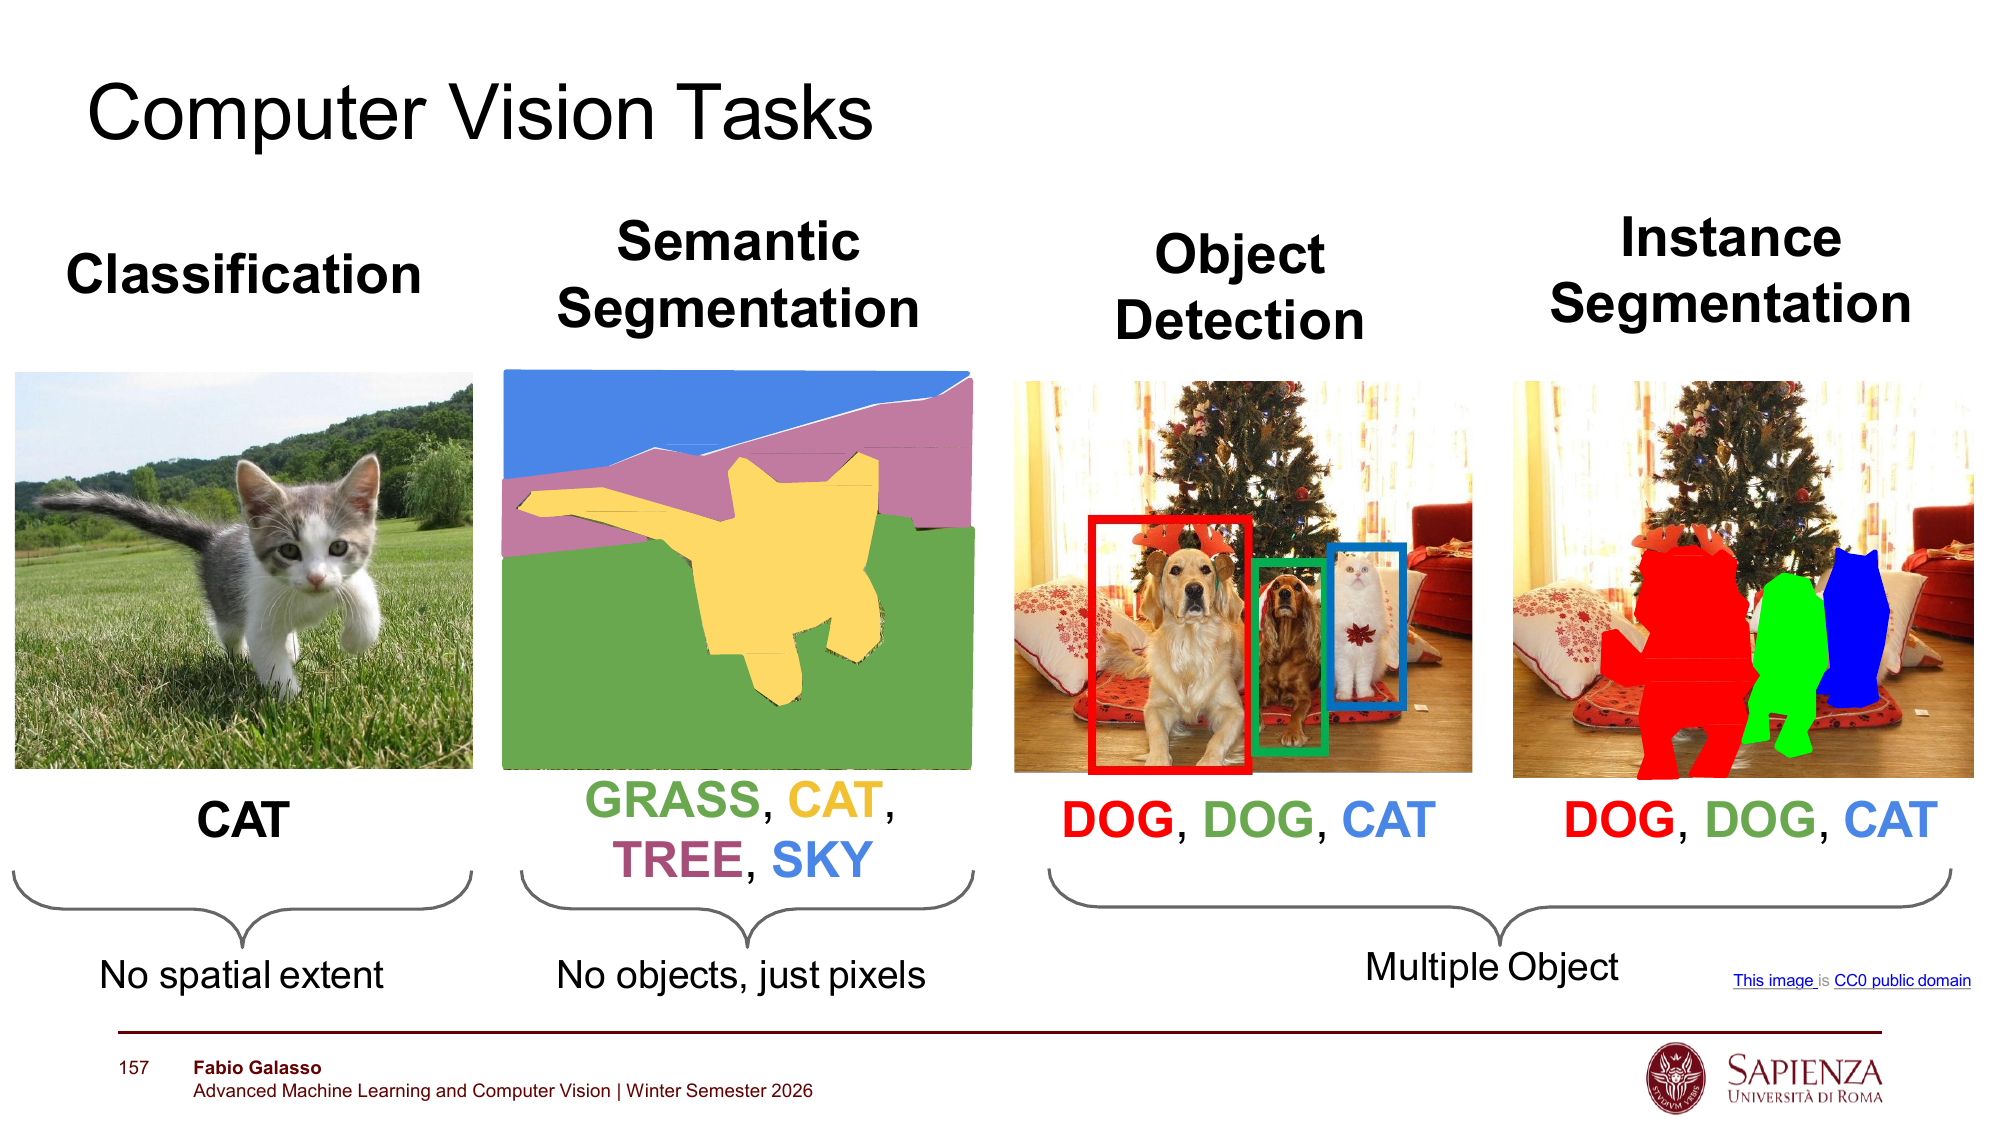
\includegraphics[width=0.95\textwidth]{Pictures/det_seg_tasks.png}
    \caption{The four core vision tasks (from course slides~\cite{galasso2025detection}). Classification predicts one label; semantic segmentation labels every pixel; object detection returns a set of boxes; instance segmentation returns a separate mask for every object.}\label{fig:det_seg_tasks}
\end{figure}

\begin{itemize}[leftmargin=*]
    \item \textbf{Classification:} one label for the whole image, with no spatial extent.
    \item \textbf{Semantic segmentation:} one class label per pixel, but no distinction between different instances of the same class.
    \item \textbf{Object detection:} a variable-length set of bounding boxes, each with a class label.
    \item \textbf{Instance segmentation:} a mask for every individual object, combining detection with pixel-level separation.
\end{itemize}

Semantic segmentation mixes two kinds of categories. \textbf{Things} are countable objects with a constrained shape and a separate identity (person, cat, car). \textbf{Stuff} is amorphous regions without a clear instance boundary (road, grass, sky). Things usually require object-level reasoning; stuff can often be labeled from local texture.

\section{Semantic Segmentation}

\subsection{Sliding Window and Its Limits}

The simplest approach classifies the center pixel of every image patch with a CNN. The patch provides the local context, and the network outputs the class of its center. This is conceptually simple but very inefficient: adjacent patches overlap heavily, and the shared features are recomputed for every pixel. The receptive field also limits how much context each prediction can see.

\begin{Notebox}
\textbf{Why sliding windows are not enough:} a single pixel is ambiguous without context, but a large patch makes the per-pixel cost explode. The fully convolutional approach solves both problems by computing all pixel scores in one shared forward pass.
\end{Notebox}

\subsection{Fully Convolutional Networks}

A \textbf{Fully Convolutional Network (FCN)} replaces the final fully connected layers with convolutions and produces a score tensor of shape $C \times H \times W$, where $C$ is the number of classes. Applying an argmax over the channel dimension yields the predicted class for every pixel:
\begin{equation}
    \hat{y}[i,j] = \arg\max_{c \in \{1,\dots,C\}} s_c[i,j].
\end{equation}
The network is trained with a per-pixel cross-entropy loss. Computing full-resolution convolutions everywhere is expensive, so practical FCNs use a contracting path that downsamples the image and an expanding path that upsamples the coarse scores back to the original resolution.

\begin{figure}[htbp]
    \centering
    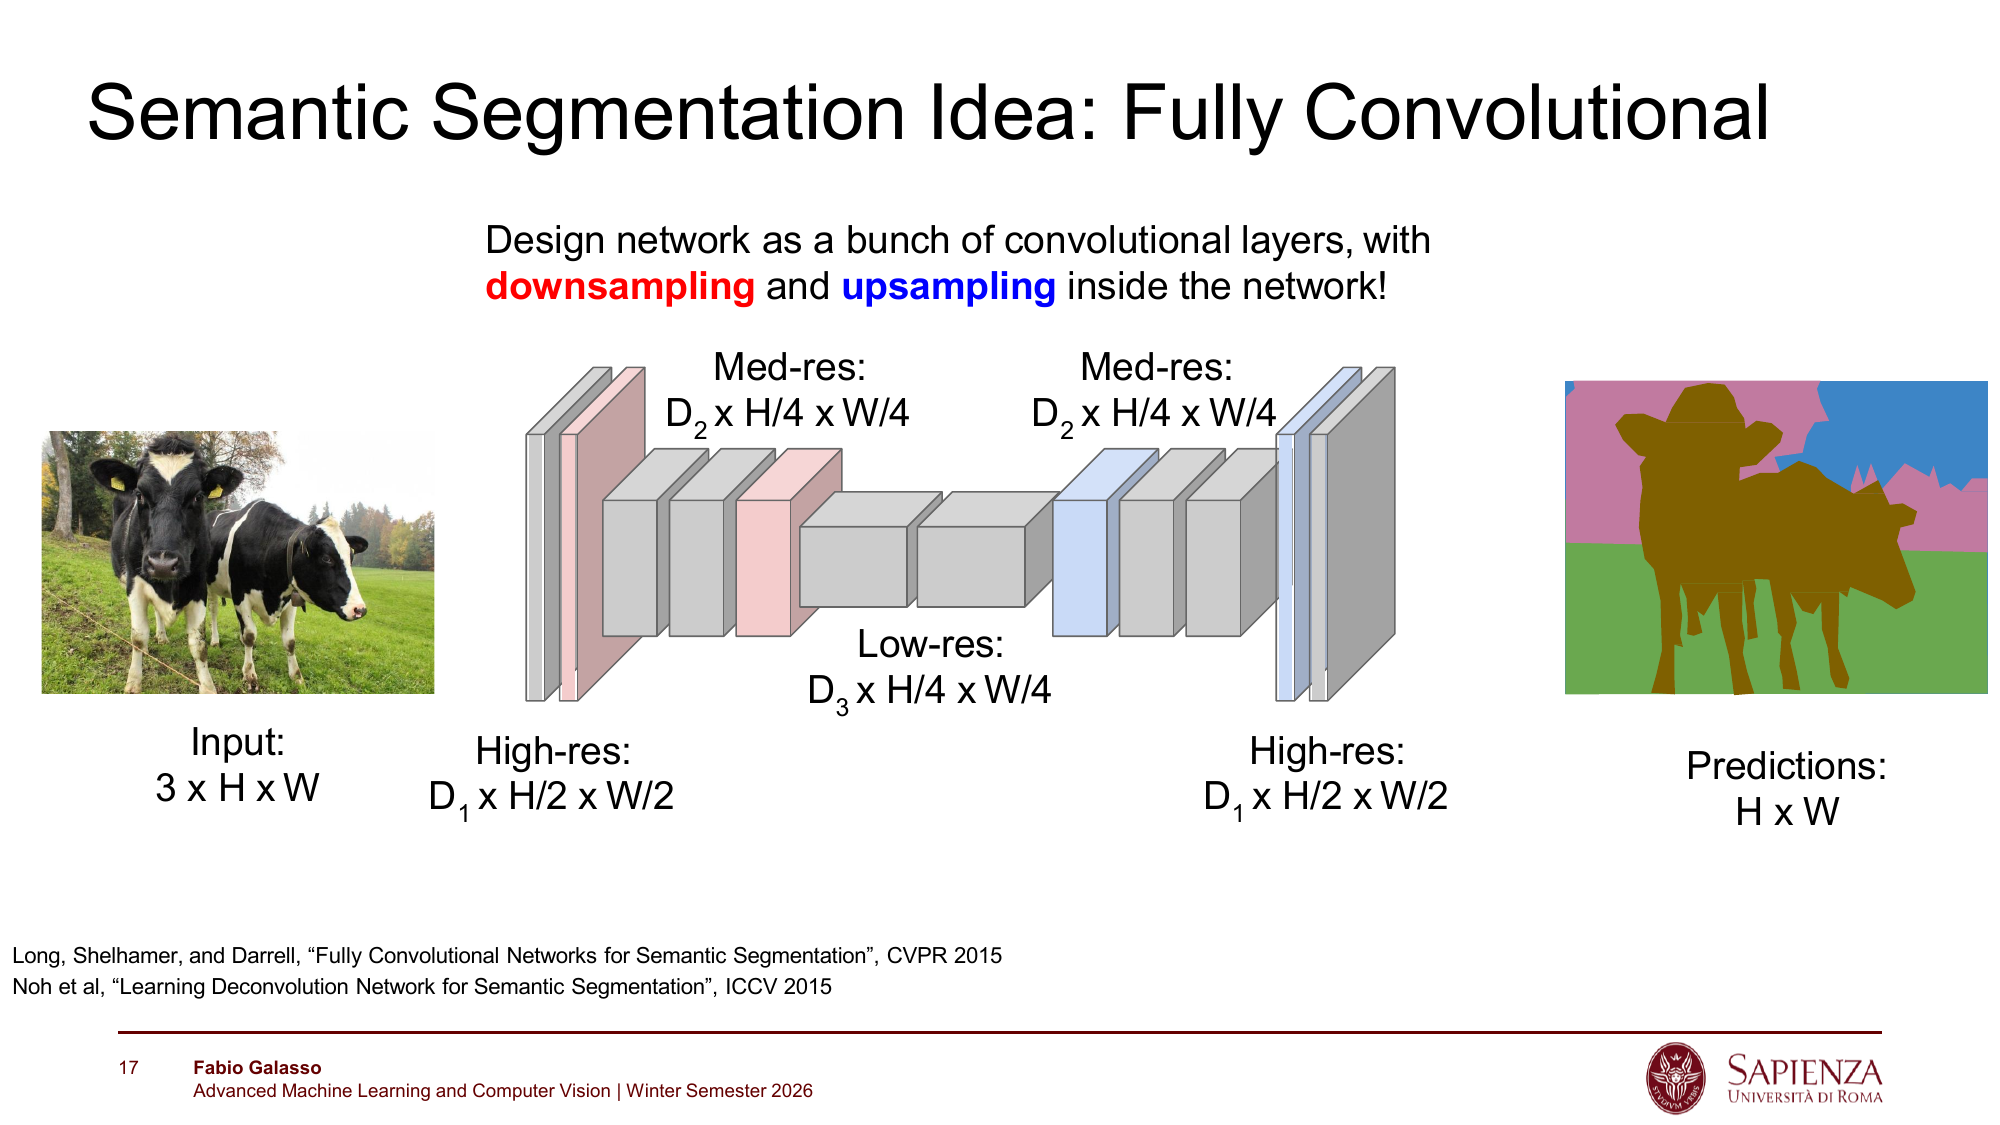
\includegraphics[width=0.92\textwidth]{Pictures/det_seg_fcn.png}
    \caption{Fully convolutional segmentation with downsampling and upsampling (from course slides~\cite{galasso2025detection}). The network produces low-resolution semantic scores and then upsamples them to a full-resolution prediction map.}\label{fig:det_seg_fcn}
\end{figure}

\subsection{Upsampling: Nearest Neighbor, Bed of Nails, Unpooling, and Transpose Convolution}

Downsampling increases the field of view but discards spatial detail. The expanding path must restore the resolution. Upsampling methods split into fixed operations and learnable operations.

\paragraph{Fixed upsampling.}
\begin{itemize}[leftmargin=*]
    \item \textbf{Nearest neighbor:} copy each input value to a block of output positions. For a $2 \times 2$ input and a scale factor of $2$, every value is replicated in a $2 \times 2$ block, producing a $4 \times 4$ output. It has no learnable parameters and is very cheap, but the result is blocky.
    \item \textbf{Bed of nails:} place each input value at one position inside its output block and fill all remaining positions with zeros. The output is sparse, like nails on a board. It is also parameter-free; a convolution is usually applied afterwards to fill the gaps.
    \item \textbf{Max unpooling:} remember the indices selected by max pooling and scatter each activation back to its winning position. This preserves the exact location of the strongest response and is the index-aware version of unpooling.
\end{itemize}
Nearest neighbor, bed of nails, and max unpooling are all \emph{fixed}: they rearrange activations without learning a filter.

\paragraph{Learnable upsampling.}
\textbf{Transpose convolution} learns an upsampling filter instead of using fixed copies, zeros, or indices. It is the transpose of the matrix that represents the corresponding convolution.

For a 1D input $[p,q]$ and a kernel $[u,v,w]$, the transpose convolution produces
\[
[p u,\; p v,\; p w + q u,\; q v,\; q w],
\]
and one boundary value is cropped to obtain exactly twice the input length. In matrix form, if a convolution is written as
\begin{equation}
    \vec{x} * \vec{a} = X \vec{a},
\end{equation}
then the transpose convolution is
\begin{equation}
    \vec{x} *^{T} \vec{a} = X^{T} \vec{a}.
\end{equation}
The name comes from this transpose, not from a new kernel family. The operation is also called \emph{deconvolution} in some libraries, although it is not the mathematical inverse of convolution. Because its kernel is trained with the rest of the network, transpose convolution can learn a smoother and more task-specific upsampling than nearest neighbor or bed of nails.

\begin{figure}[htbp]
    \centering
    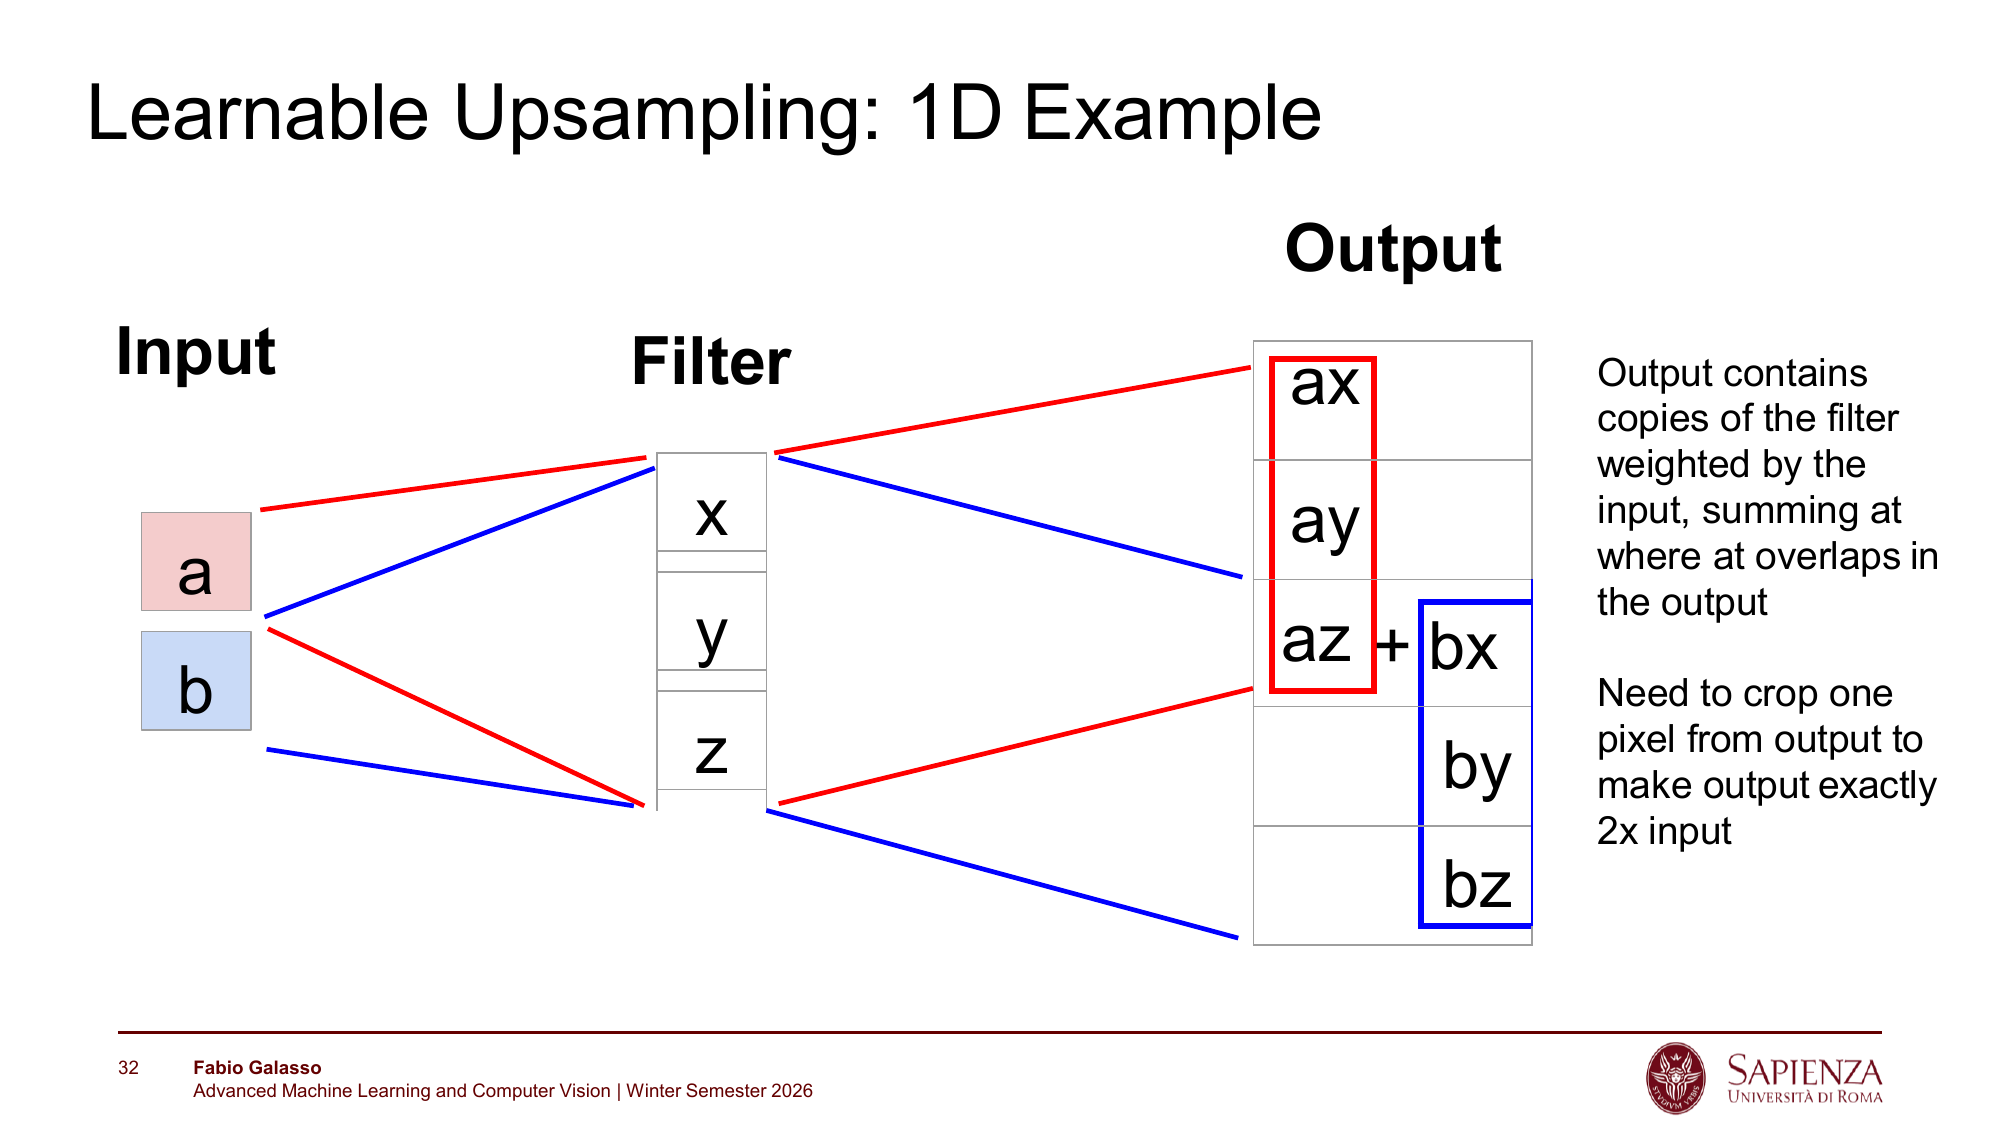
\includegraphics[width=0.82\textwidth]{Pictures/det_seg_transpose_conv.png}
    \caption{Learnable upsampling with a 1D transpose convolution (from course slides~\cite{galasso2025detection}). Each input value multiplies the learned kernel, and overlapping contributions are summed in the output.}\label{fig:det_seg_transpose_conv}
\end{figure}

\subsection{U-Net}

\textbf{U-Net} combines the contracting and expanding paths with \textbf{skip connections}. The encoder repeatedly applies convolutions and pooling, increasing the field of view while reducing the resolution. The decoder upsamples the features back to the input resolution. At each resolution, a skip connection concatenates the high-resolution encoder features with the upsampled decoder features, so the decoder receives both semantic context and precise spatial detail.

\begin{figure}[htbp]
    \centering
    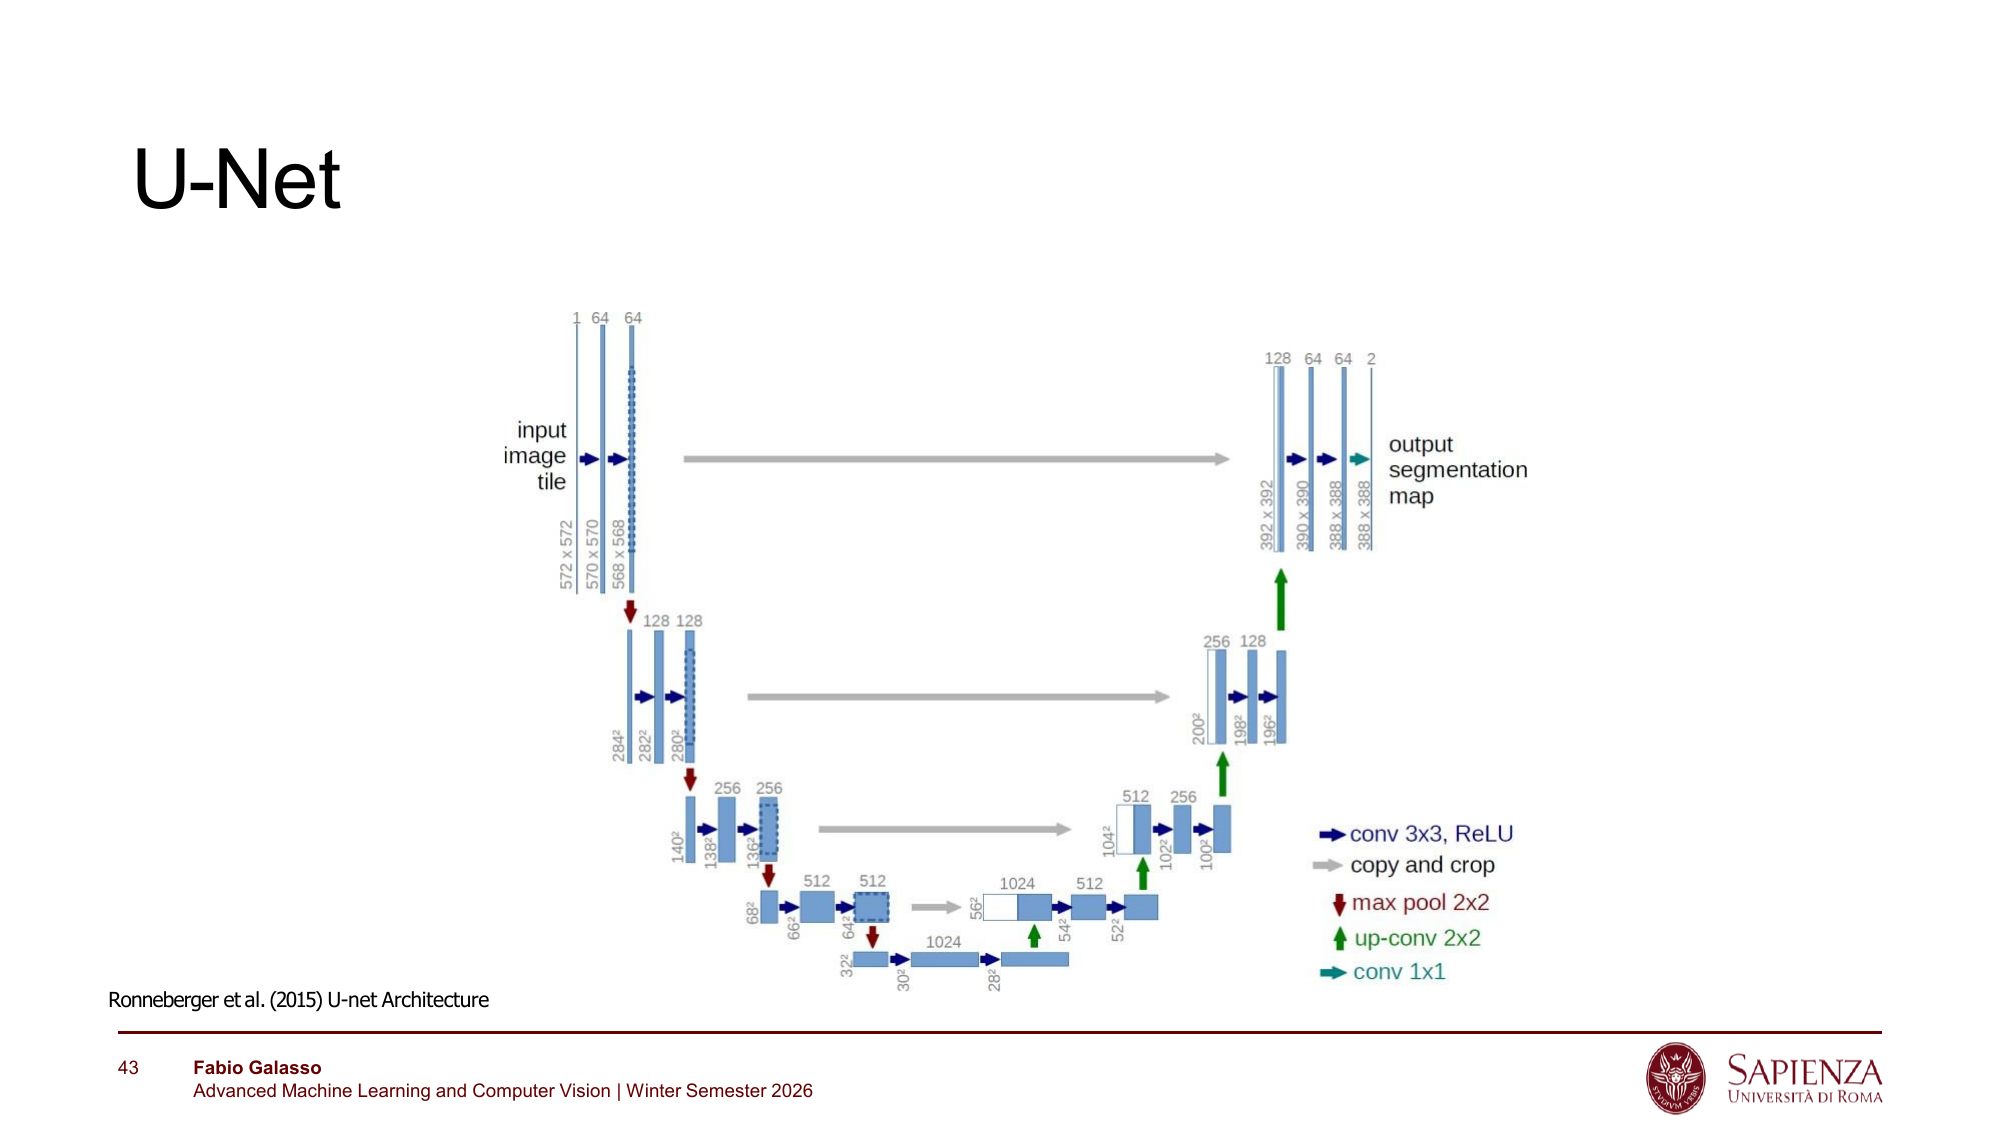
\includegraphics[width=0.78\textwidth]{Pictures/det_seg_unet.png}
    \caption{The U-Net architecture (from course slides~\cite{galasso2025detection, ronneberger2015u}). The contracting path extracts context; the expanding path restores resolution; skip connections transfer fine spatial information across the two paths.}\label{fig:det_seg_unet}
\end{figure}

\subsection{Evaluation and Annotation}

Pixel accuracy is a misleading metric when one class dominates the image: a model that predicts only ``background'' can score very high. The standard semantic-segmentation metric is the \textbf{Intersection over Union (IoU)} for each class $c$:
\begin{equation}
    \mathrm{IoU}_c = \frac{|P_c \cap G_c|}{|P_c \cup G_c|},
\end{equation}
where $P_c$ is the set of pixels predicted as class $c$ and $G_c$ is the ground-truth set. The reported \textbf{mean IoU} averages $\mathrm{IoU}_c$ over classes and images. Per-class accuracy is also reported, because it gives equal weight to rare classes.

Annotation is expensive: precise boundaries are hard to draw, and labeling every pixel produces a heavy-tailed distribution over classes. A common compromise is to annotate a small set of \emph{thing} classes and mark everything else as ``Other''. Standard benchmarks include PASCAL VOC and COCO.

\section{Object Detection}

\subsection{Single Object: Classification plus Localization}

For one object, the network must output both a class and a box. A standard design shares a backbone, then splits into two heads:
\begin{itemize}[leftmargin=*]
    \item a \textbf{classification head} with a Softmax over classes;
    \item a \textbf{regression head} with four coordinates $(x,y,w,h)$ for the box.
\end{itemize}
The model is trained with a multi-task loss:
\begin{equation}
    \mathcal{L} = \mathcal{L}_{\text{cls}} + \lambda \mathcal{L}_{\text{box}},
\end{equation}
where $\mathcal{L}_{\text{cls}}$ is the classification cross-entropy and $\mathcal{L}_{\text{box}}$ is a regression loss (L2 or smooth L1) between the predicted and ground-truth box. The backbone is usually pre-trained on ImageNet and then fine-tuned, which is the same transfer-learning recipe used in Chapter~\ref{ch:convnets}.

A box can be parameterized by its center and size $(x,y,w,h)$ or by its corners $(x_{\min},y_{\min},x_{\max},y_{\max})$. The regression head predicts an offset from a reference box, and the loss is often the \textbf{smooth L1} loss, which behaves quadratically for small errors and linearly for large ones:
\begin{equation}
    \mathrm{smooth}_{L_1}(e) =
    \begin{cases}
        0.5 e^2 & \text{if } |e| < 1, \\
        |e| - 0.5 & \text{otherwise}.
    \end{cases}
\end{equation}
This makes the detector less sensitive to outliers than plain L2 regression.

\subsection{Multiple Objects}

A real image contains a variable number of objects, so the network cannot use a fixed output size. The classical pipeline applies a CNN to many candidate crops and classifies each crop as one of the object classes or as \emph{background}. Two post-processing tools are essential.

\paragraph{Intersection over Union.} For two boxes $A$ and $B$,
\begin{equation}
    \mathrm{IoU}(A,B) = \frac{|A \cap B|}{|A \cup B|}.
\end{equation}
IoU measures how well a predicted box overlaps the ground-truth box and is also used to decide whether a detection is a true positive.

\paragraph{Non-Maximum Suppression (NMS).} Many overlapping boxes propose the same object. NMS sorts the boxes by confidence, keeps the highest-scoring one, suppresses every remaining box whose IoU with the kept box exceeds a threshold (for example, $0.5$), and repeats with the next highest-scoring box. In practice, low-confidence boxes are discarded first, and NMS is applied per class so that two different classes can overlap.

\begin{keywordbox}
\textbf{Detection output is a set, not a fixed vector.} A detector must return a variable number of boxes, one per object, and must learn to reject background regions. This is why detection needs both a classification score and a box regression, plus a post-processing step such as NMS.
\end{keywordbox}

\subsection{Region Proposals and R-CNN}

\textbf{R-CNN} (Regions with CNN features) separates the problem into two stages. First, an external proposal method such as \textbf{selective search} generates a few thousand class-agnostic region candidates. Second, each region is warped to a fixed size (for example, $227 \times 227$), passed through a CNN, and classified with a linear SVM; a separate regressor refines the box. The CNN is pre-trained on ImageNet and then fine-tuned on the detection data.

R-CNN is accurate but slow: the CNN is run separately on every proposal, so thousands of forward passes are needed for a single image. The features of overlapping regions are also recomputed many times. Training is multi-stage (CNN, SVM, box regressor), which makes the pipeline cumbersome.

\subsection{Fast R-CNN and RoI Pooling}

\textbf{Fast R-CNN} removes the repeated CNN passes. The whole image is processed once by the backbone, producing a shared feature map. Each proposal is then projected onto this feature map and converted into a fixed-size region descriptor by \textbf{RoI pooling}: the region is divided into a grid (for example, $7 \times 7$), and max pooling is applied inside each cell. Classification and box regression share this descriptor, so the network is trained with a multi-task loss. Because all proposals reuse the same feature map, Fast R-CNN is much faster than R-CNN and can be trained end-to-end.

\begin{figure}[htbp]
    \centering
    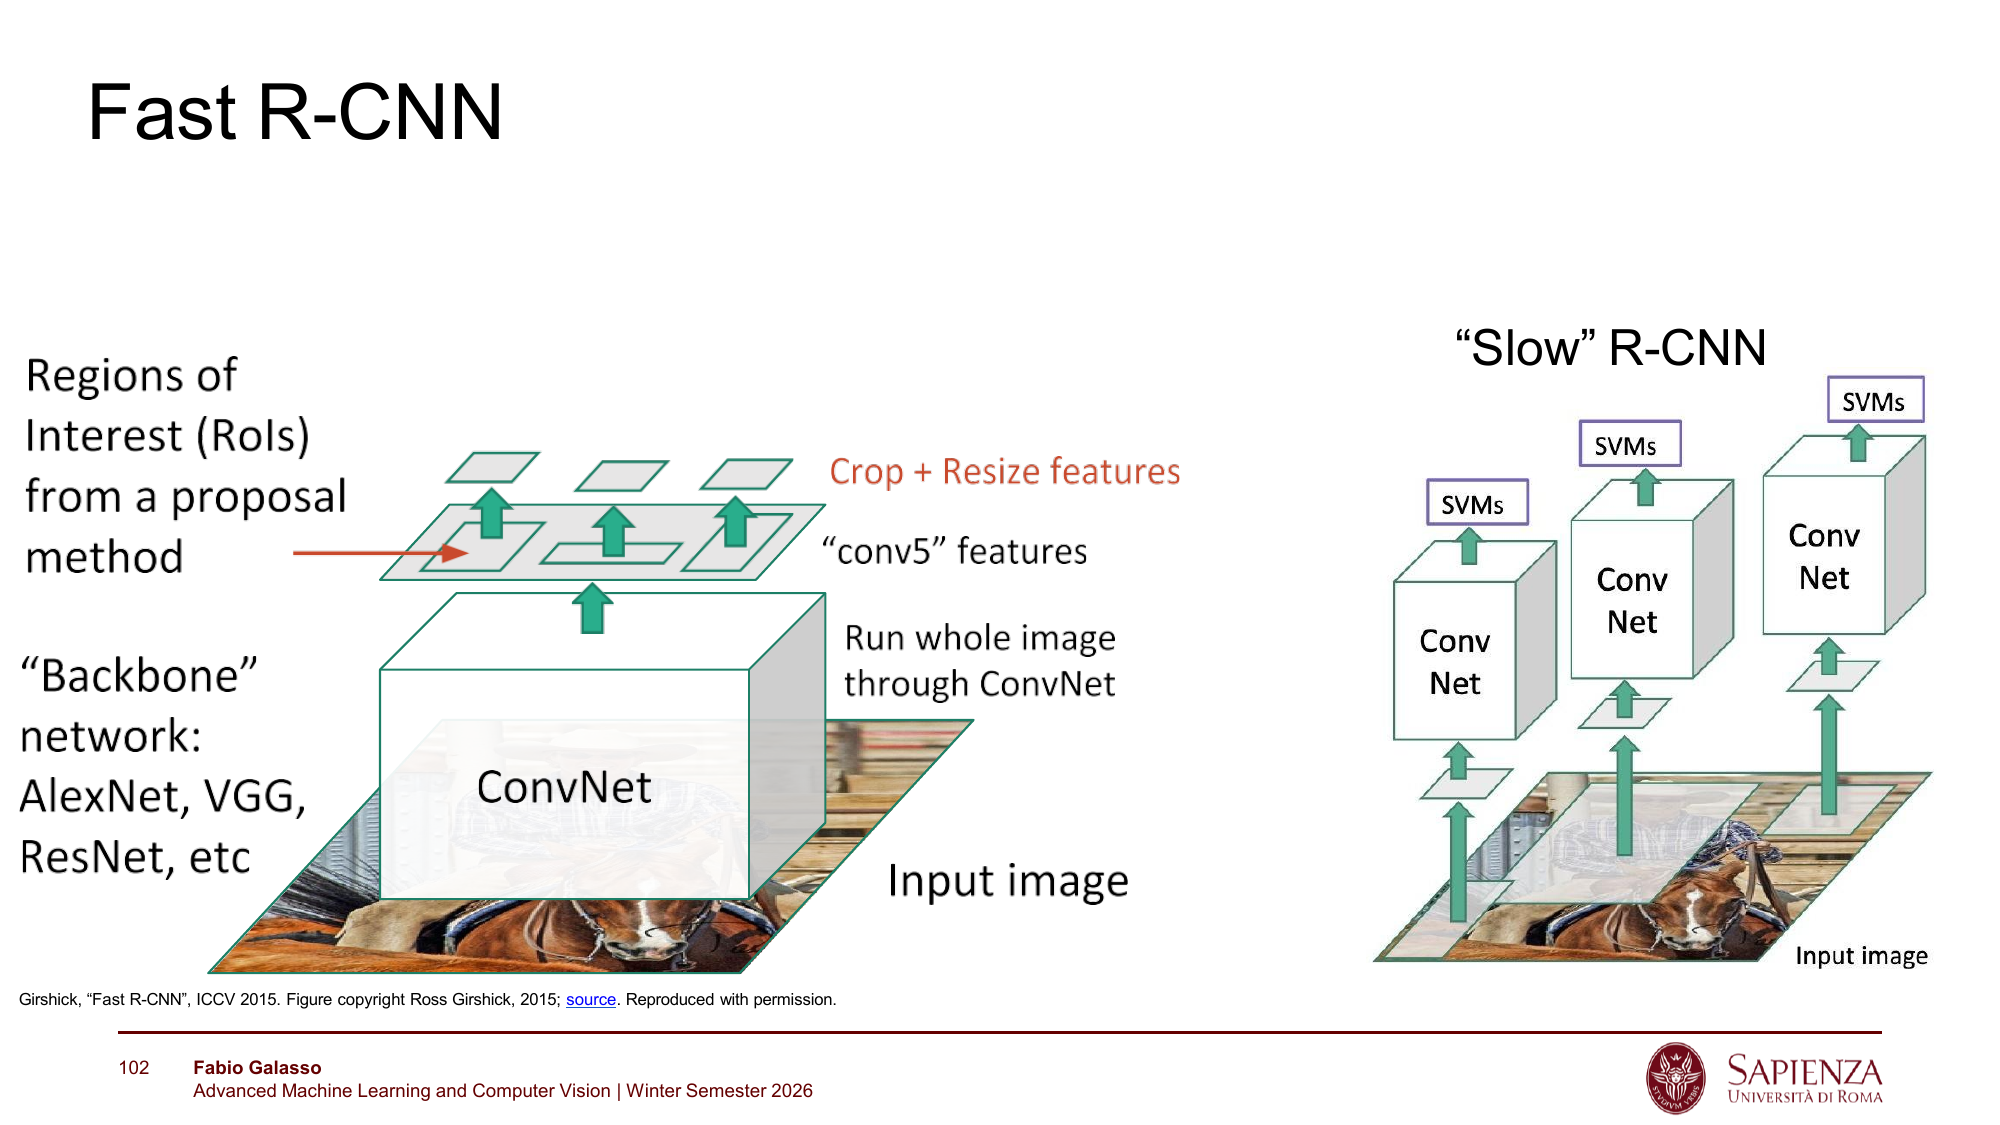
\includegraphics[width=0.92\textwidth]{Pictures/det_seg_fast_rcnn.png}
    \caption{Fast R-CNN versus the original R-CNN (from course slides~\cite{galasso2025detection, girshick2015fast}). Fast R-CNN runs the backbone once and crops region features from the shared feature map; the original R-CNN runs a separate CNN for every proposal.}\label{fig:det_seg_fast_rcnn}
\end{figure}

RoI pooling has a subtle flaw: projecting a proposal onto the discrete feature grid requires ``snapping'' to cell boundaries, which slightly misaligns the features. \textbf{RoI Align} fixes this by sampling at regular points inside each region and using bilinear interpolation, without snapping. At each sample point $(x,y)$, the feature is a weighted combination of its four neighboring grid cells:
\begin{equation}
    f(x,y) = (1-\Delta_x)(1-\Delta_y) f_{00}
    + \Delta_x(1-\Delta_y) f_{10}
    + (1-\Delta_x)\Delta_y f_{01}
    + \Delta_x\Delta_y f_{11},
\end{equation}
where $\Delta_x,\Delta_y$ are the fractional offsets inside the cell. This detail is important for mask prediction, where pixel-level alignment matters.

\begin{figure}[htbp]
    \centering
    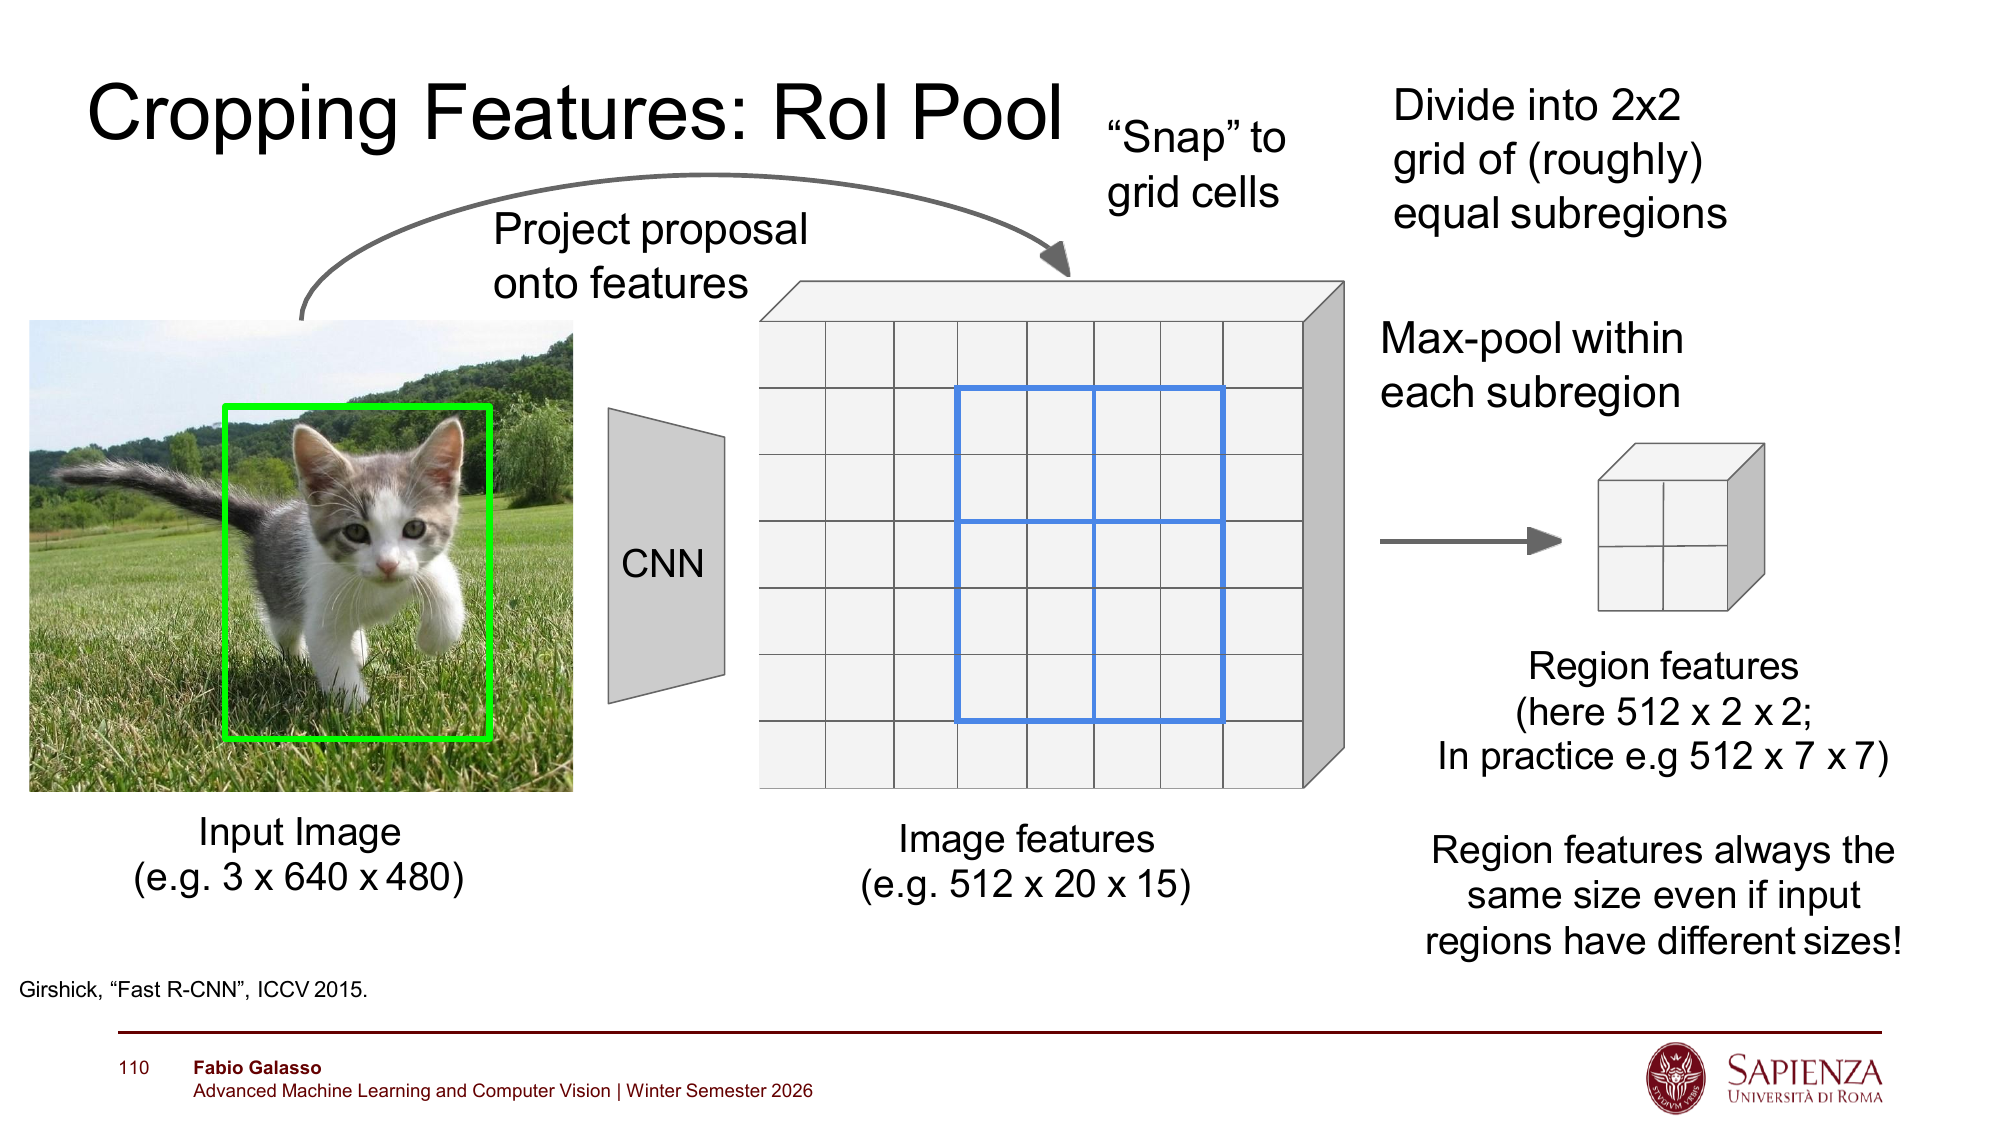
\includegraphics[width=0.90\textwidth]{Pictures/det_seg_roi_pool.png}
    \caption{RoI pooling (from course slides~\cite{galasso2025detection, girshick2015fast}). A proposal is projected onto the feature map, divided into a fixed grid, and max-pooled into a constant-size region descriptor.}\label{fig:det_seg_roi_pool}
\end{figure}

\subsection{Faster R-CNN and the Region Proposal Network}

Fast R-CNN still depends on an external proposal method, and that proposal step dominates the runtime. \textbf{Faster R-CNN} makes the CNN produce the proposals itself with a \textbf{Region Proposal Network (RPN)}.

The RPN slides a small network over the feature map. At every spatial location it considers $K$ \textbf{anchor boxes} of different sizes and aspect ratios, and predicts:
\begin{itemize}[leftmargin=*]
    \item an \textbf{objectness} score for each anchor (object versus background);
    \item four \textbf{box transforms} that move the anchor toward the ground-truth box.
\end{itemize}
Anchors are assigned a positive label if their IoU with a ground-truth box is above a threshold (for example, $0.7$), and a negative label if it is below a lower threshold (for example, $0.3$); the anchors in between are ignored. The RPN loss is a sum of an objectness term and a box-regression term:
\begin{equation}
    \mathcal{L}_{\text{RPN}} = \frac{1}{N_{\text{obj}}}\sum_i \mathcal{L}_{\text{obj}}(p_i,p_i^*) + \lambda\frac{1}{N_{\text{reg}}}\sum_i p_i^*\,\mathcal{L}_{\text{reg}}(t_i,t_i^*),
\end{equation}
where $p_i^*=1$ only for positive anchors. The highest-scoring proposals (typically around 300) are kept, NMS is applied, and the survivors are passed to the second stage, which performs RoI pooling/align, classification, and box refinement. Faster R-CNN is therefore a \textbf{two-stage detector}: the first stage proposes, the second stage classifies and refines. It is trained jointly with four losses: RPN objectness, RPN box regression, final classification, and final box regression.

\begin{figure}[htbp]
    \centering
    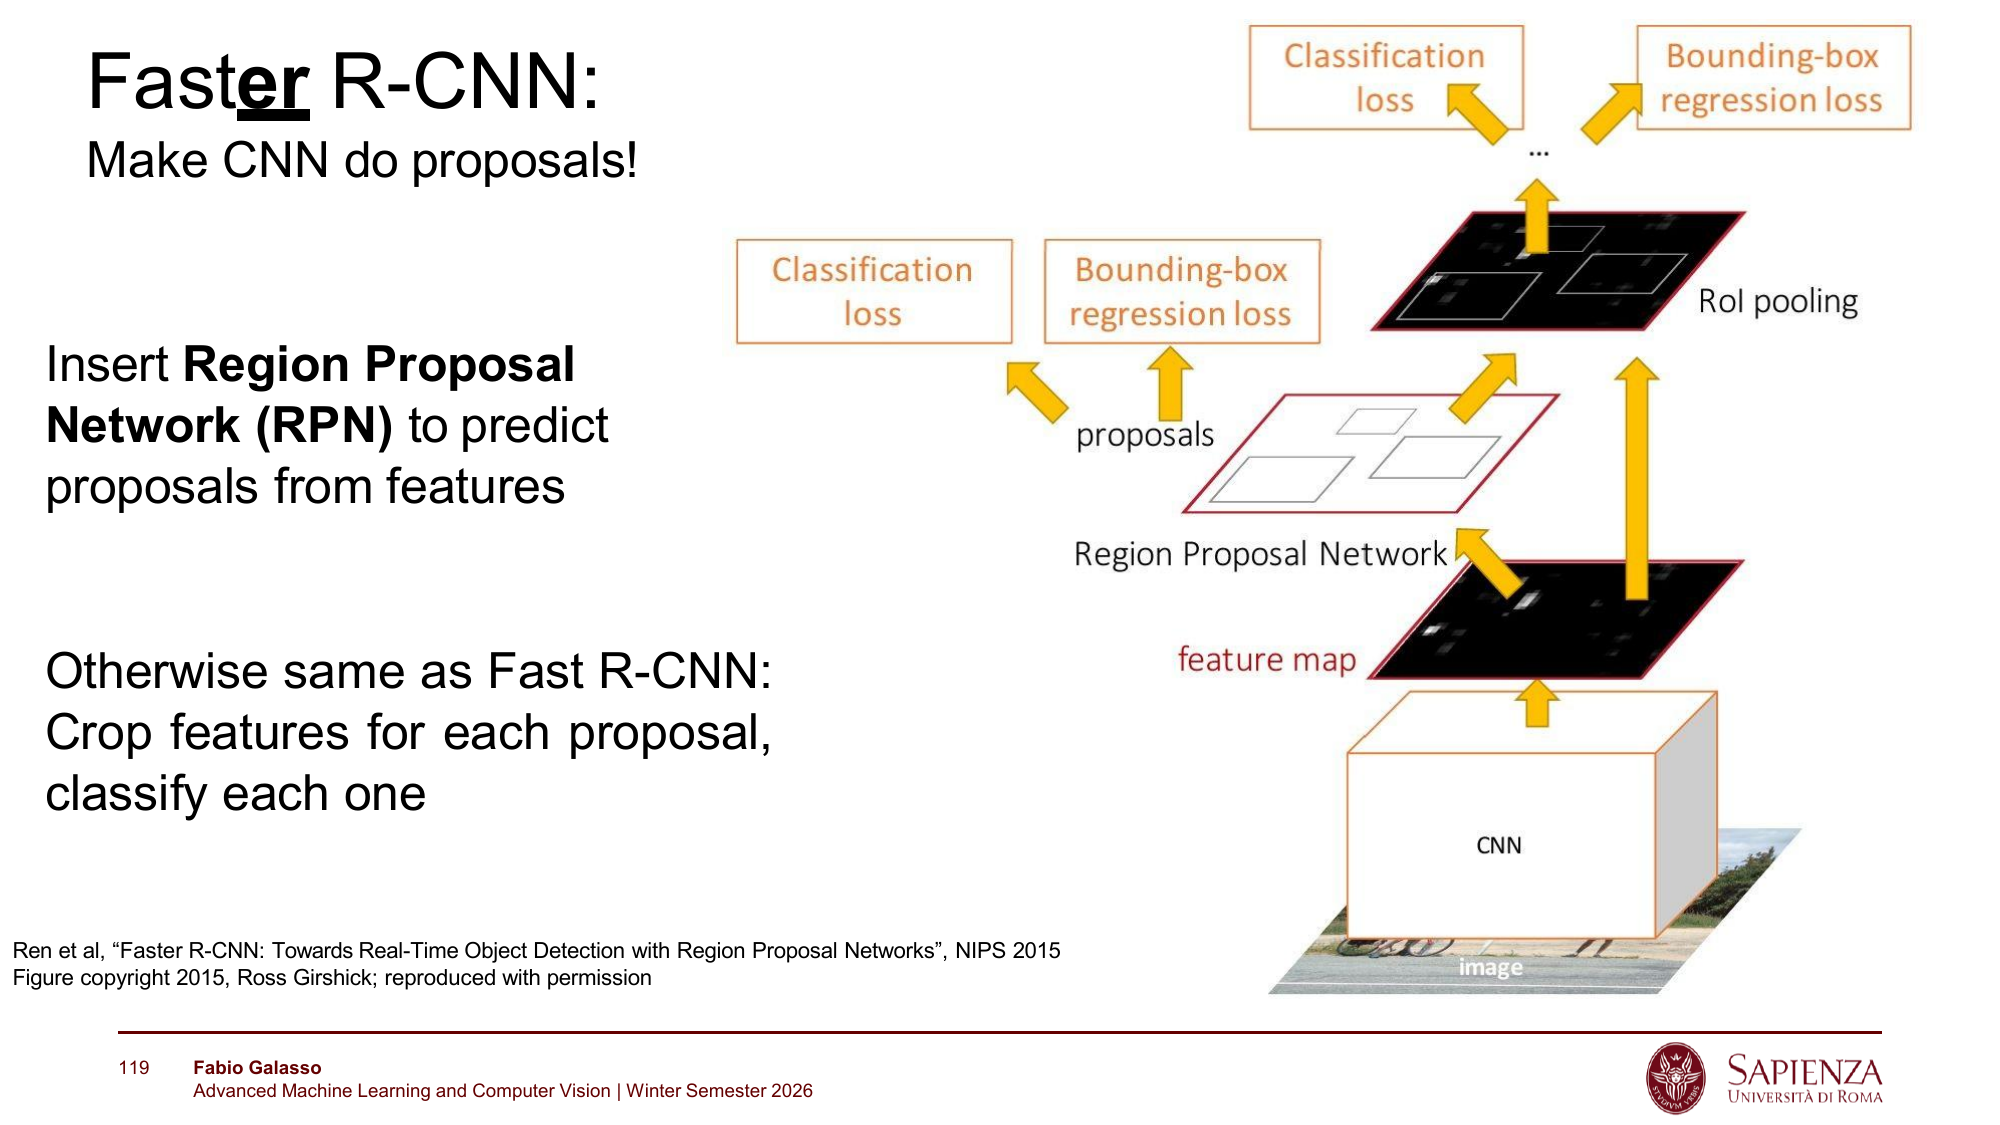
\includegraphics[width=0.92\textwidth]{Pictures/det_seg_faster_rcnn.png}
    \caption{Faster R-CNN with a Region Proposal Network (from course slides~\cite{galasso2025detection, ren2015faster}). The RPN predicts proposals directly from the shared feature map; the second stage crops features with RoI pooling and predicts classes and box offsets.}\label{fig:det_seg_faster_rcnn}
\end{figure}

\subsection{Single-Stage Detectors: YOLO, SSD, and RetinaNet}

Two-stage detectors are accurate but relatively slow because proposals and per-region heads are sequential. \textbf{Single-stage detectors} predict classes and boxes directly from a dense feature map in one pass.

\textbf{YOLO} divides the image into an $S \times S$ grid. Each cell predicts $B$ bounding boxes, a confidence $P(\text{object})$ for each box, four box coordinates, and class probabilities. The output tensor therefore has shape
\begin{equation}
    S \times S \times \left(B\cdot 5 + C\right),
\end{equation}
where the factor $5$ accounts for the four box coordinates plus the objectness score. The confidence used at inference is
\begin{equation}
    \text{score} = P(\text{object}) \cdot \mathrm{IoU}(\text{pred},\text{gt}),
\end{equation}
and the class-specific score multiplies it by $P(\text{class}\mid\text{object})$. The final detection is obtained by thresholding the score and applying NMS. Because the whole image is processed once, YOLO is much faster than R-CNN-style pipelines.

\begin{figure}[htbp]
    \centering
    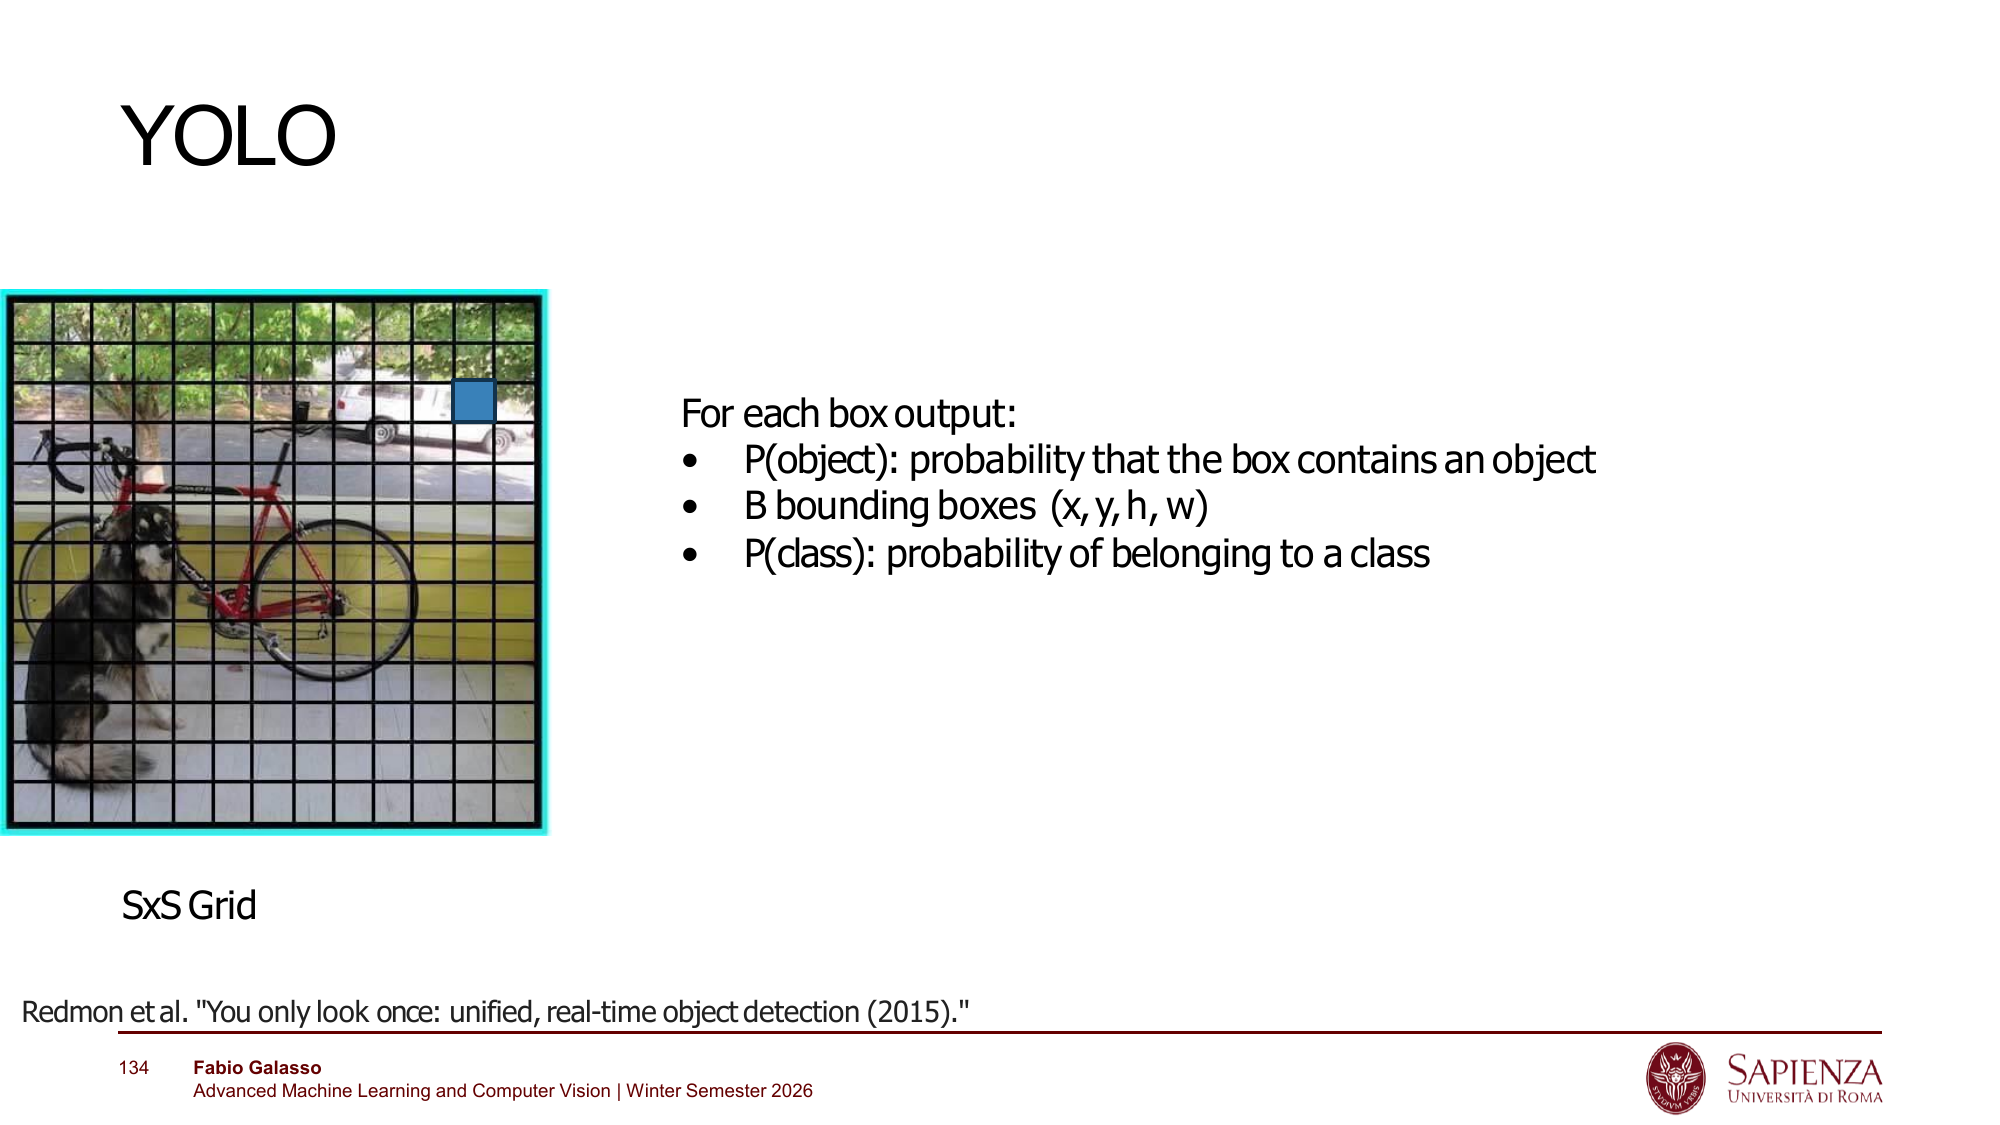
\includegraphics[width=0.82\textwidth]{Pictures/det_seg_yolo.png}
    \caption{YOLO's $S \times S$ grid (from course slides~\cite{galasso2025detection, redmon2016you}). Each cell predicts objectness, box coordinates, and class probabilities for a small set of boxes.}\label{fig:det_seg_yolo}
\end{figure}

\textbf{SSD} applies similar predictions at multiple feature-map resolutions, which gives it access to both small and large objects; each resolution uses a set of default boxes with different scales and aspect ratios. \textbf{RetinaNet} keeps the single-stage design but introduces the \textbf{focal loss} to counter the extreme imbalance between easy background anchors and rare foreground objects:
\begin{equation}
    \mathrm{FL}(p_t) = -\alpha_t (1-p_t)^{\gamma}\log p_t,
\end{equation}
where $p_t$ is the probability assigned to the correct class and $\gamma>0$ down-weights easy examples. With $\gamma=2$, well-classified background anchors contribute almost no gradient, so the detector can focus on hard foreground examples without sampling heuristics.

\subsection{DETR: Detection as Set Prediction}

\textbf{DETR} (Detection Transformer) removes anchors and NMS entirely. A CNN backbone extracts a set of image features, a Transformer encoder-decoder processes them, and a fixed set of learned \textbf{object queries} produces box predictions and class labels. The number of queries is fixed (for example, 100); each query predicts either an object or the special \emph{no-object} class $\varnothing$. The prediction is a \emph{set}, so the model is trained with a \textbf{bipartite matching} between predicted and ground-truth objects:
\begin{equation}
    \hat{\sigma} = \arg\min_{\sigma} \sum_{i} \mathcal{L}_{\text{match}}\left(y_i, \hat{y}_{\sigma(i)}\right),
\end{equation}
where $\sigma$ is a permutation of the predictions and the matching cost combines the class probability with a box distance (L1 and/or GIoU). The matched pairs are then used in a Hungarian loss that combines classification and box regression:
\begin{equation}
    \mathcal{L}_{\text{Hungarian}} = \sum_{i=1}^{N}
    \left[-\log \hat{p}_{\hat{\sigma}(i)}(c_i)
    + \mathbb{1}_{[c_i\neq\varnothing]}\,\mathcal{L}_{\text{box}}\left(b_i,\hat{b}_{\hat{\sigma}(i)}\right)\right].
\end{equation}
Because each ground-truth object is matched to exactly one prediction, DETR does not need NMS. The price is a fixed set size and slower convergence; later variants such as Deformable DETR address the small-object and training-speed limitations.

\begin{figure}[htbp]
    \centering
    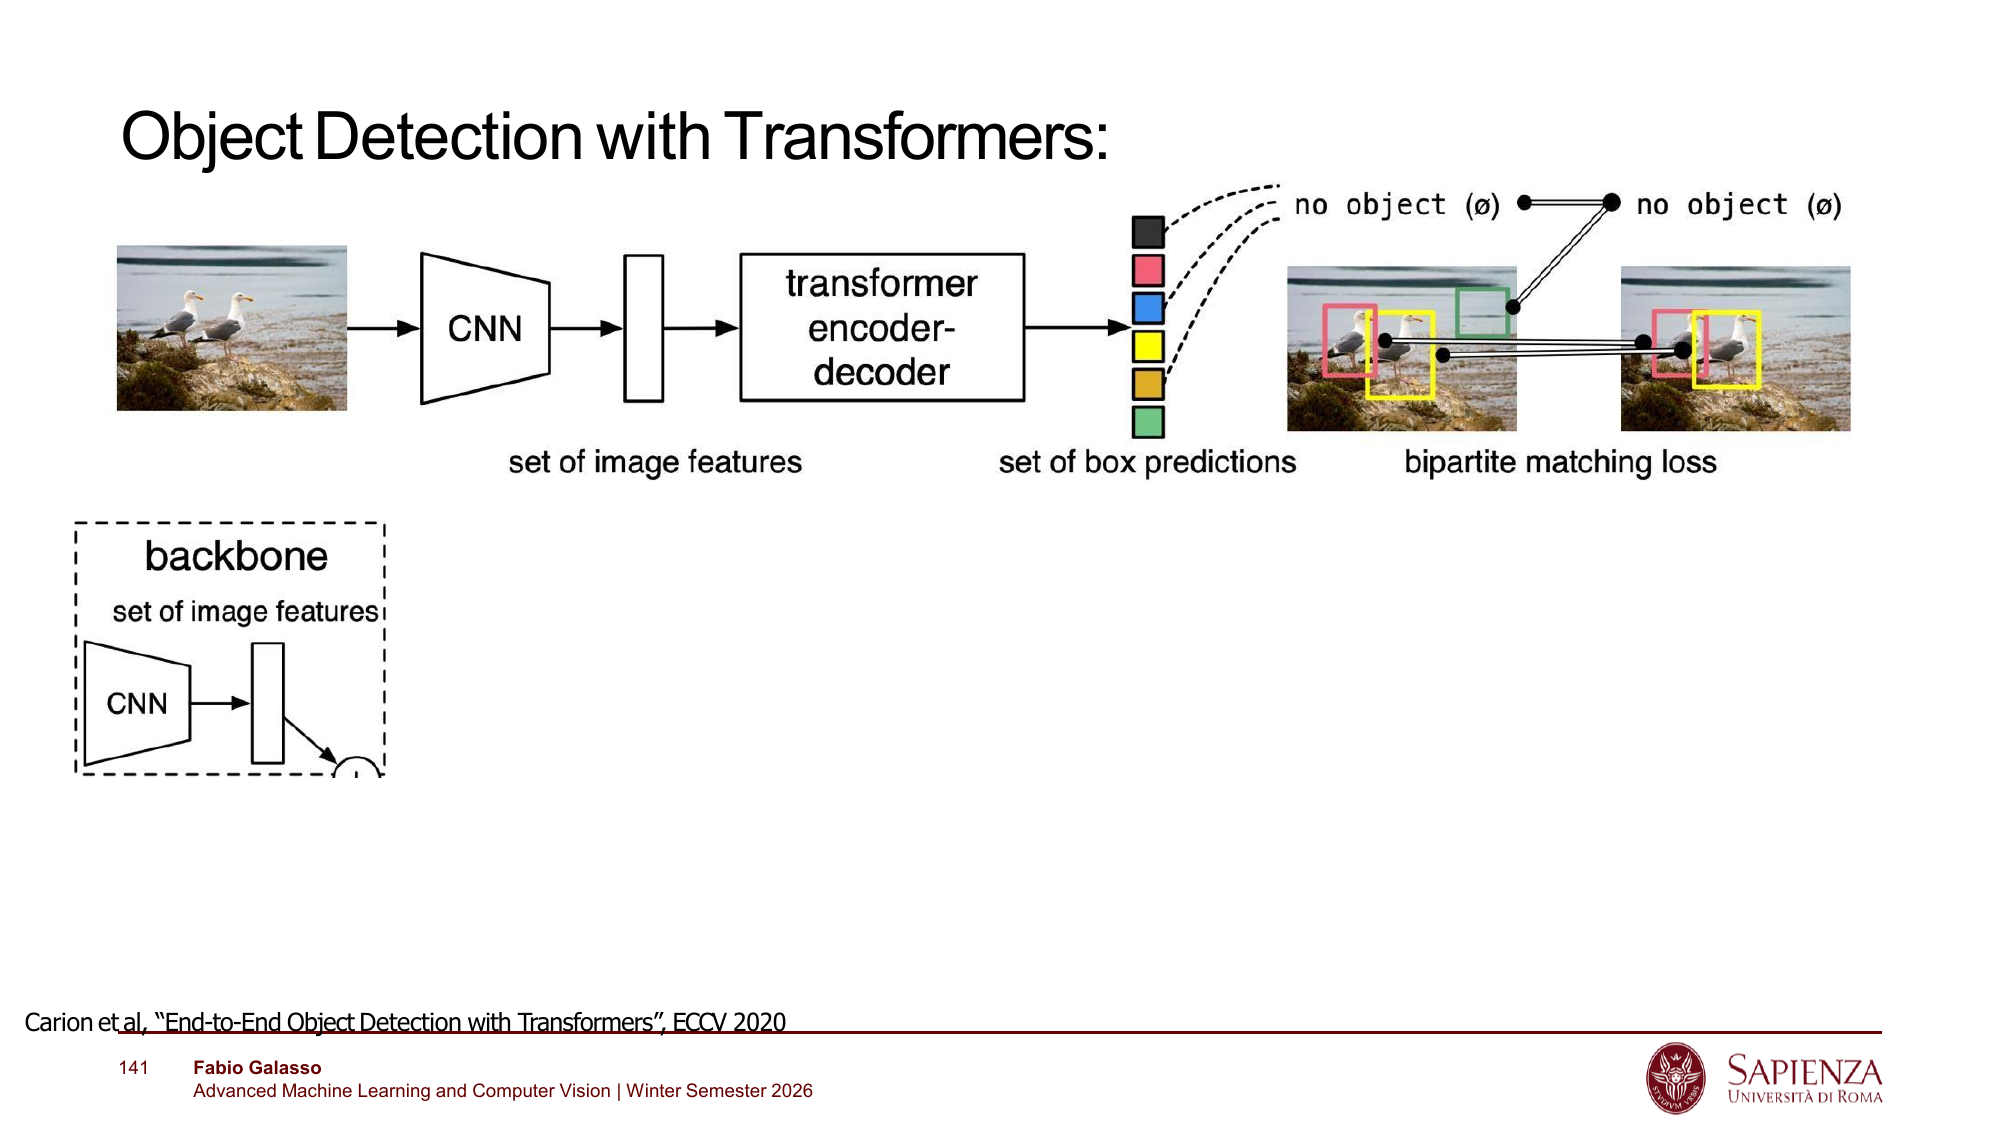
\includegraphics[width=0.92\textwidth]{Pictures/det_seg_detr.png}
    \caption{DETR (from course slides~\cite{galasso2025detection, carion2020end}). A CNN backbone and a Transformer encoder-decoder directly output a set of box predictions; bipartite matching assigns predictions to ground-truth objects during training.}\label{fig:det_seg_detr}
\end{figure}

\subsection{Evaluation: Mean Average Precision}

Detection is evaluated with \textbf{mean Average Precision (mAP)}. For each class, predictions are sorted by confidence. A prediction is a true positive if its IoU with a ground-truth box exceeds a threshold and the ground-truth box has not already been matched. Precision and recall are computed at every confidence level, producing a precision-recall curve; the \textbf{Average Precision (AP)} is the area under this curve. The \textbf{mAP} averages AP over classes. COCO reports AP averaged over IoU thresholds from $0.50$ to $0.95$ in steps of $0.05$, which rewards both accurate classification and precise localization.

\section{Instance Segmentation}

\subsection{Mask R-CNN}

\textbf{Mask R-CNN} extends Faster R-CNN with a third output branch. For every region proposal, the network predicts:
\begin{itemize}[leftmargin=*]
    \item the class label;
    \item the bounding-box coordinates;
    \item a binary mask for the object.
\end{itemize}
The mask branch is a small convolutional network applied to each RoI after \textbf{RoI Align}. It outputs a $C \times 28 \times 28$ mask, one channel per class, and the mask loss is computed only on positive RoIs. The full loss is
\begin{equation}
    \mathcal{L} = \mathcal{L}_{\text{cls}} + \mathcal{L}_{\text{box}} + \mathcal{L}_{\text{mask}},
\end{equation}
where $\mathcal{L}_{\text{mask}}$ is a per-pixel binary cross-entropy on the ground-truth mask of the matched class. Predicting one mask per class avoids competition between classes: the mask branch does not have to choose the class, it only has to delineate the object. The classification and box branches decide \emph{what} and \emph{where}; the mask branch decides \emph{which pixels}.

\begin{figure}[htbp]
    \centering
    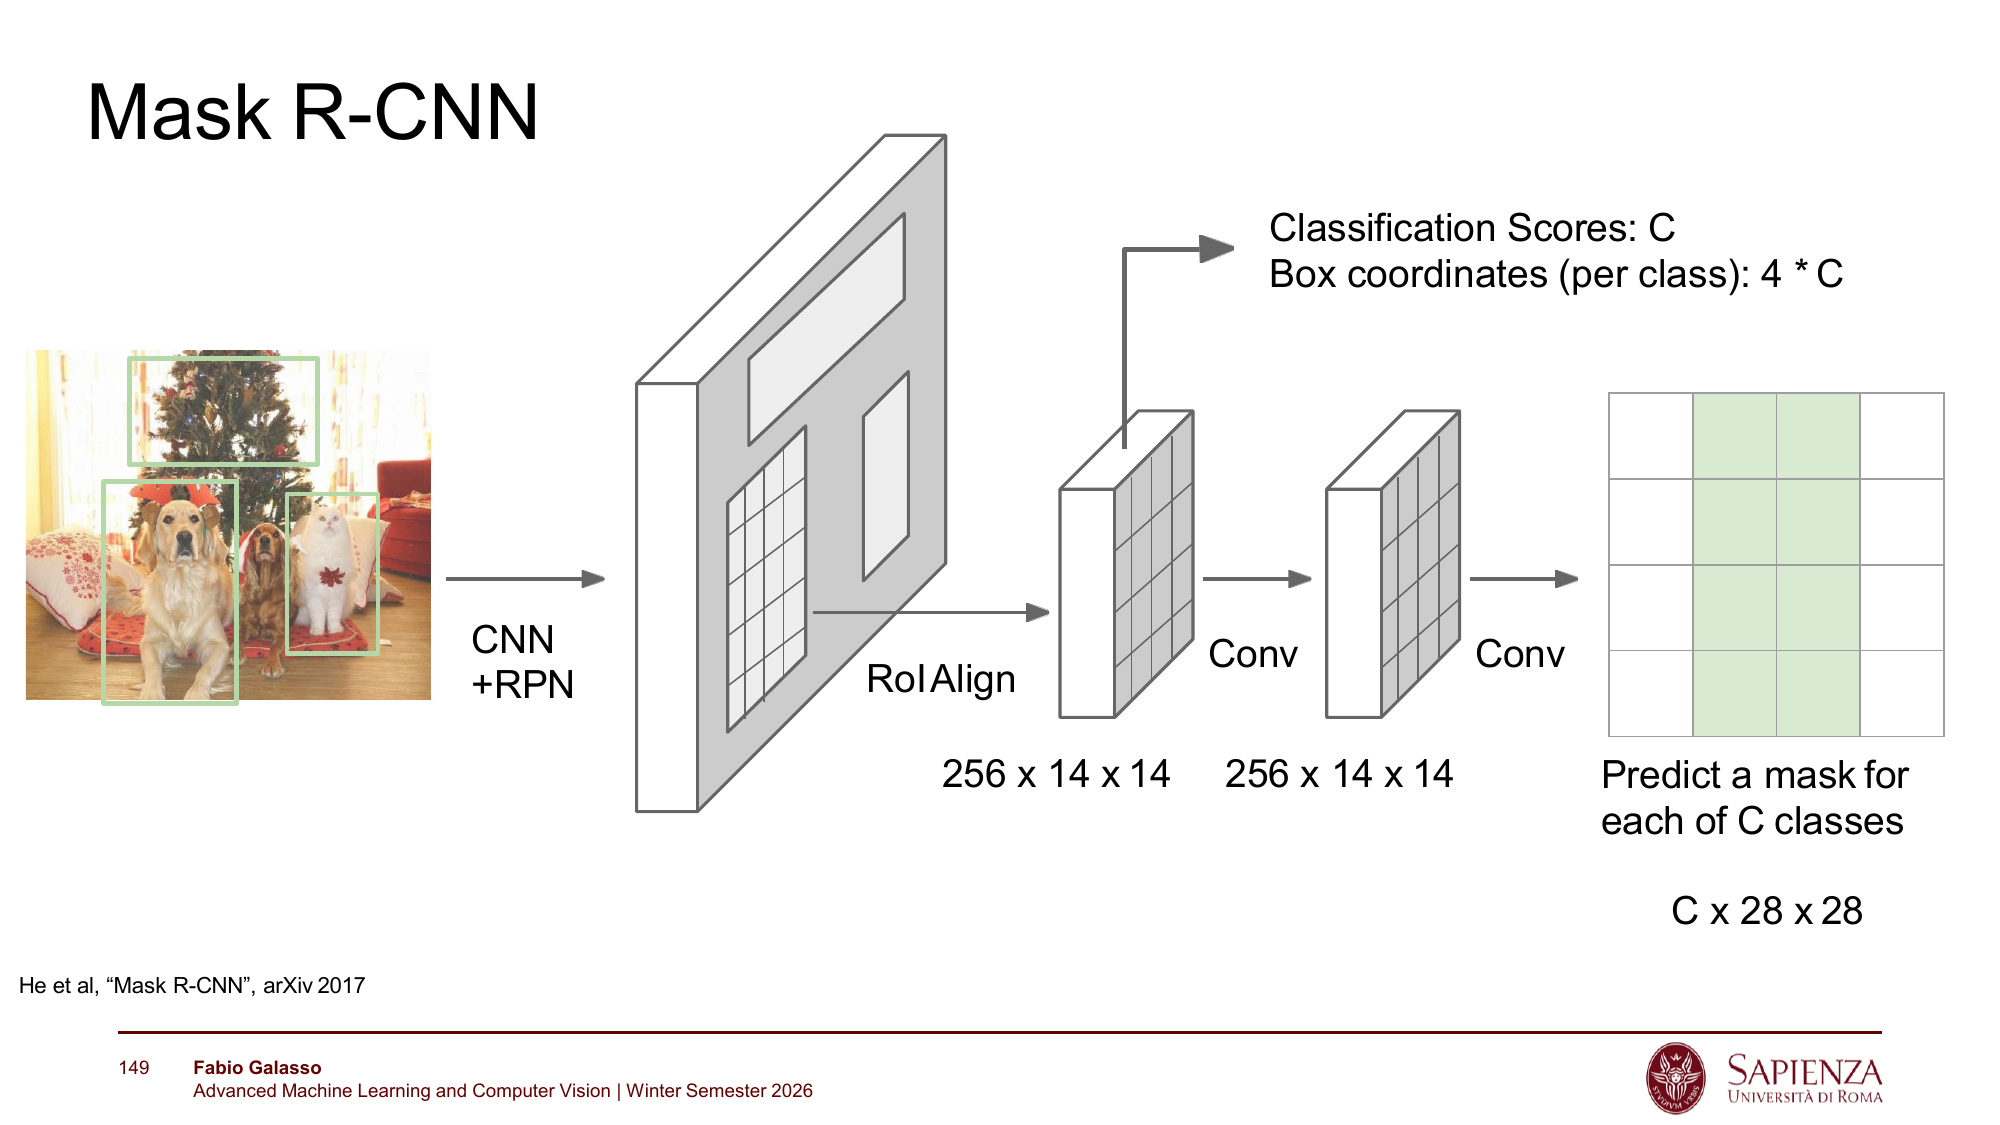
\includegraphics[width=0.92\textwidth]{Pictures/det_seg_mask_rcnn.png}
    \caption{Mask R-CNN (from course slides~\cite{galasso2025detection, he2017mask}). A mask branch runs in parallel with classification and box regression, predicting a per-class $28 \times 28$ mask for every RoI after RoI Align.}\label{fig:det_seg_mask_rcnn}
\end{figure}

RoI Align is especially important here: mask prediction requires sub-pixel alignment between the proposal and the feature map, and the coarse snapping of RoI pooling would blur the mask boundaries. The same architecture can also predict human pose keypoints by replacing the mask branch with a keypoint head.

\section{Beyond 2D}

The same detection machinery extends beyond bounding boxes:
\begin{itemize}[leftmargin=*]
    \item \textbf{Dense captioning:} detect regions and describe each one with a sentence.
    \item \textbf{Dense video captioning:} localize and describe events in a video.
    \item \textbf{Scene graphs:} detect objects and predict the relationships between them.
    \item \textbf{3D object detection:} predict 3D boxes from images or point clouds.
    \item \textbf{3D shape prediction:} reconstruct voxel grids, point clouds, or meshes; Mesh R-CNN combines detection with mesh generation.
\end{itemize}
These are extensions of the core ideas, not separate detection paradigms: a backbone extracts features, a head predicts geometry and semantics, and a matching or post-processing step turns the predictions into a structured output.

\newpage
\section{Recap: Key Concepts}

The chapter follows the path from coarse image labels to dense, structured predictions: classification says \emph{what}, detection says \emph{what and where}, semantic segmentation says \emph{which class per pixel}, and instance segmentation says \emph{which pixels belong to which object}. The architecture evolves from sliding windows to shared convolutional features, region proposals, single-stage detectors, and Transformer-based set prediction.

\begin{table}[htbp]
\centering
\small
\renewcommand{\arraystretch}{1.05}
\begin{tabular}{p{0.20\textwidth} p{0.36\textwidth} p{0.32\textwidth}}
\toprule
\textbf{Concept} & \textbf{Key idea} & \textbf{Formula / rule} \\
\midrule
Task taxonomy & Classification, semantic segmentation, detection, instance segmentation & label, pixel map, boxes, masks \\
Semantic segmentation & One class per pixel; sliding windows are inefficient & $\hat{y}[i,j]=\arg\max_c s_c[i,j]$ \\
FCN & Convolutional scores for all pixels & $C \times H \times W$ output \\
Fixed upsampling & Nearest neighbor, bed of nails, max unpooling & parameter-free rearrangement \\
Transpose convolution & Learnable upsampling & $\vec{x}*^T\vec{a}=X^T\vec{a}$ \\
U-Net & Encoder-decoder with skip connections & high-resolution detail + context \\
IoU & Overlap between prediction and ground truth & $|P\cap G|/|P\cup G|$ \\
Object detection & Box plus class per object & $(x,y,w,h)$ + class score \\
NMS & Remove duplicate boxes & keep highest score, suppress $\mathrm{IoU}>\tau$ \\
R-CNN family & Proposals, shared features, RPN & selective search $\to$ RoI pool $\to$ two-stage \\
YOLO / SSD / RetinaNet & Single-stage dense prediction & fast, no proposal step \\
DETR & Set prediction with Transformer & bipartite matching, no NMS \\
Mask R-CNN & Detection + per-object mask & $C\times28\times28$ mask per RoI \\
mAP & Average precision over classes & area under precision-recall \\
\bottomrule
\end{tabular}
\caption{One-page recap of the key concepts in this chapter.}\label{tab:ch6_recap}
\end{table}

\begin{InsightBox}
\textbf{The one-sentence version:} detection and segmentation replace the single image label with structured outputs; shared convolutional features, region proposals, anchor-free or Transformer set prediction, and mask branches progressively answer \emph{what} is where, and which pixels belong to it.
\end{InsightBox}
